\appendix

\chapter{Backpropagation} \label{backprop}

Backpropagation is the flow of information from the outputs of the network back through the network. Once the cost function has been computed
finding the gradient of the loss with respect to each trainable parameter shows which direction the parameter can be shifted to decrease 
the loss function.. This derivation of the backpropagation algorithm is based on that found in \textit{Artificial intelligence I}~\cite{Art_Int}.
In the derivations below:
\begin{itemize}
  \item $J(\vec{\theta})_k$ is the cost function for the $kth$ sample in the training set
  \item $w_{i \to j}$ is the weight between node $i$ and node $j$
  \item $a_j$ is the value computed by the node $j$ pre-activation ($\sum_{k} w_{k \to j} z_k$)
  \item $z_j$ and $y_j$ are the values post-activation ($\sigma(a_j)$), for non-output and output nodes respectively
\end{itemize}

The value to be calculated for each weight (per sample) is $\frac{\partial J(\vec{\theta})_k}{\partial w_{i \to j}}$. To do this we use the chain rule
of differentiation:
\begin{align}
  \frac{\partial J(\vec{\theta})_k}{\partial w_{i \to j}} & = \frac{\partial J(\vec{\theta})_k}{\partial a_j} \frac{\partial a_j}{\partial w_{i \to j}} \\
  & = \frac{\partial J(\vec{\theta})_k}{\partial a_j} z_i
\end{align}

Then for weights connected to the output nodes:
\begin{align}
  \frac{\partial J(\vec{\theta})_k}{\partial w_{i \to j}} & = \frac{\partial J(\vec{\theta})_k}{\partial a_j} z_i \\
  & = \frac{\partial J(\vec{\theta})_k}{\partial y_j} \frac{\partial y_j}{\partial a_j} z_i
\end{align}

If our loss function is differentiable with respect to $y_j$, and $y_j$ is differetiable with respect to $a_j$ then we can calculate this.  
For backpropagation to work all our loss and activation functions must have this property. Thankfully all the loss and activation functions 
shown in this dissertation do have that property and so work correctly with backpropagation.

Once the gradients are computed for the weights in the output layer it is possible to calculate them for the next layer, and then the
layer after that, etc., as the errors are backpropagated through the network. The computation for the hidden layers is slightly more 
complicated:
\begin{align}
  \frac{\partial J(\vec{\theta})_k}{\partial w_{i \to j}} & = \frac{\partial J(\vec{\theta})_k}{\partial a_j} z_i \\
  & = \left( \sum_{k \in K} \frac{\partial J(\vec{\theta})_k}{\partial a_k} \frac{\partial a_k}{\partial a_j} \right) z_i
\end{align}
\begin{center}
  \textit{where K is the set of all nodes $j$ is connected to in the next layer}
\end{center}

By definition:
\begin{align}
  \frac{\partial a_k}{\partial a_j} & = \frac{\partial}{\partial a_j} \left( \sum_{i} w_{i \to k} z_i \right) \\
  & = \frac{\partial}{\partial a_j} \left( \sum_{i} w_{i \to k} \sigma(a_i) \right) \\
  & = w_{j \to k} \sigma'(a_j)
\end{align}

Therefore, for hidden layers:
\begin{align}
  \frac{\partial J(\vec{\theta})_k}{\partial w_{i \to j}} & = \left( \sum_{k \in K} w_{j \to k} \frac{\partial J(\vec{\theta})_k}{\partial a_k} \right) \sigma'(a_j) z_i
\end{align}

As the errors are moving backward through the network, and all nodes $k$ are in the layer after $j$, $\frac{\partial J(\vec{\theta})_k}{\partial a_k}$
has already been computed and so this gradient can be calculated.

\chapter{Derivation of VAE loss} \label{vae_loss}

\begin{align}
  \log p(x) & = \log \int p(x|z)p(z) dz &\text{Law of total probability}\\
  & = \log \int p(x|z)p(z) \frac{q(z|x)}{q(z|x)} dz\\
  & = \log\left(\mathbb{E}_q \left[\frac{p(x|z)p(z)}{q(z|x)}\right]\right) \\
  & \geq \mathbb{E}_q \left[\log\frac{p(x|z)p(z)}{q(z|x)}\right] &\text{Jensen's inequality}\\
  & = \mathbb{E}_q \left[\log p(x|z) + \log\frac{p(z)}{q(z|x)}\right] \\
  & = \mathbb{E}_q [\log p(x|z)] - D_{KL}(q(z|x)||p(z))
\end{align}

\chapter{The reparameterization trick} \label{reparam}

It is not possible to backpropagate the reconstruction loss of a varitaional autoencoder through the random sampling in the latent dimension, because the drawing of
the samples is not differentiable with respect to $\vec{\mu}$ and $\vec{\sigma}$. Previously this was solved using a Monte Carlo gradient estimator, but these have 
extremely high variance and are impractical.Instead the reparameterization trick allows the Gaussian sample to be reparameterized as:
\begin{align}
  \vec{z_{i}} = \vec{\mu} + \vec{\sigma}\vec{\epsilon}
\end{align}

$\vec{\epsilon}$ is a vector of samples from the standard normal distribution $\mathcal{N}(0, 1)$. The sampling operation is now differentiable
with respect to $\vec{\mu}$ and $\vec{\sigma}$ and therefore is differentiable with respect to $\vec{\theta}$, the trainable parameters of the encoder. As the
gradients can be backpropagated through the network it is possible to train the VAE using gradient descent.

\chapter{Derivation of semi-supervised VAE loss} \label{ssvae_loss}

For labelled data the model should maximise evidence $\log p(\vec{x}, y)$:
\begingroup
\allowdisplaybreaks
\begin{align*}
  \log p(x, y) & = \log \int p(x, y, z) dz \\
  & = \log \int p(x|y, z)p(y)p(z) dz \qquad \text{Independence of $z$ and $y$}\\
  & = \log \int p(x|y, z)p(y)p(z) \frac{q(z|x, y)}{q(z|x, y)} dz\\
  & = \log\left(\mathbb{E}_q \left[\frac{p(x|y, z)p(y)p(z)}{q(z|x, y)}\right]\right) \\
  & \geq \mathbb{E}_q \left[\log\frac{p(x|y, z)p(y)p(z)}{q(z|x, y)}\right] \\
  & = \mathbb{E}_q \left[\log p(x|y, z) + \log p(y) + \log\frac{p(z)}{q(z|x, y)}\right] \\
  & = \mathbb{E}_q [\log p(x|y, z) + \log p(y)] - D_{KL}(q(z|x, y)||p(z)) \\
  & = -\mathcal{L}(x, y)
\end{align*}
\endgroup

For unlabelled data the model should maximise $\log p(\vec{x})$:
\begingroup
\allowdisplaybreaks
\begin{align*}
  \log p(x) & = \log \sum_{y} \int p(x, y, z) dz \\
  & = \log \sum_{y} \int p(x, y, z) \frac{q(z, y|x)}{q(z, y|x)} dz\\
  & = \log \sum_{y} \int p(x, y, z) \frac{q(z|x, y)q(y|x)}{q(z|x, y)q(y|x)} dz\\
  & \geq \sum_{y} q(y|x) \int q(z|x, y) \log\frac{p(x, y, z)}{q(z|x, y)q(y|x)} dz \qquad \text{Jensen's inequality}\\
  & = \sum_{y} q(y|x) \int q(z|x, y) \log\frac{p(x, y, z)}{q(z|x, y)} dz - \sum_{y} q(y|x) \log q(y|x) \int q(z|x, y) dz\\
  & = \sum_{y} q(y|x)(-\mathcal{L}(x, y)) + \mathcal{H}(q(y|x)) \\
  & = -\mathcal{U}(x, y)
\end{align*}
\endgroup

\chapter{Confusion matrices} \label{confusion}

\begin{figure}[H]
  \centering
  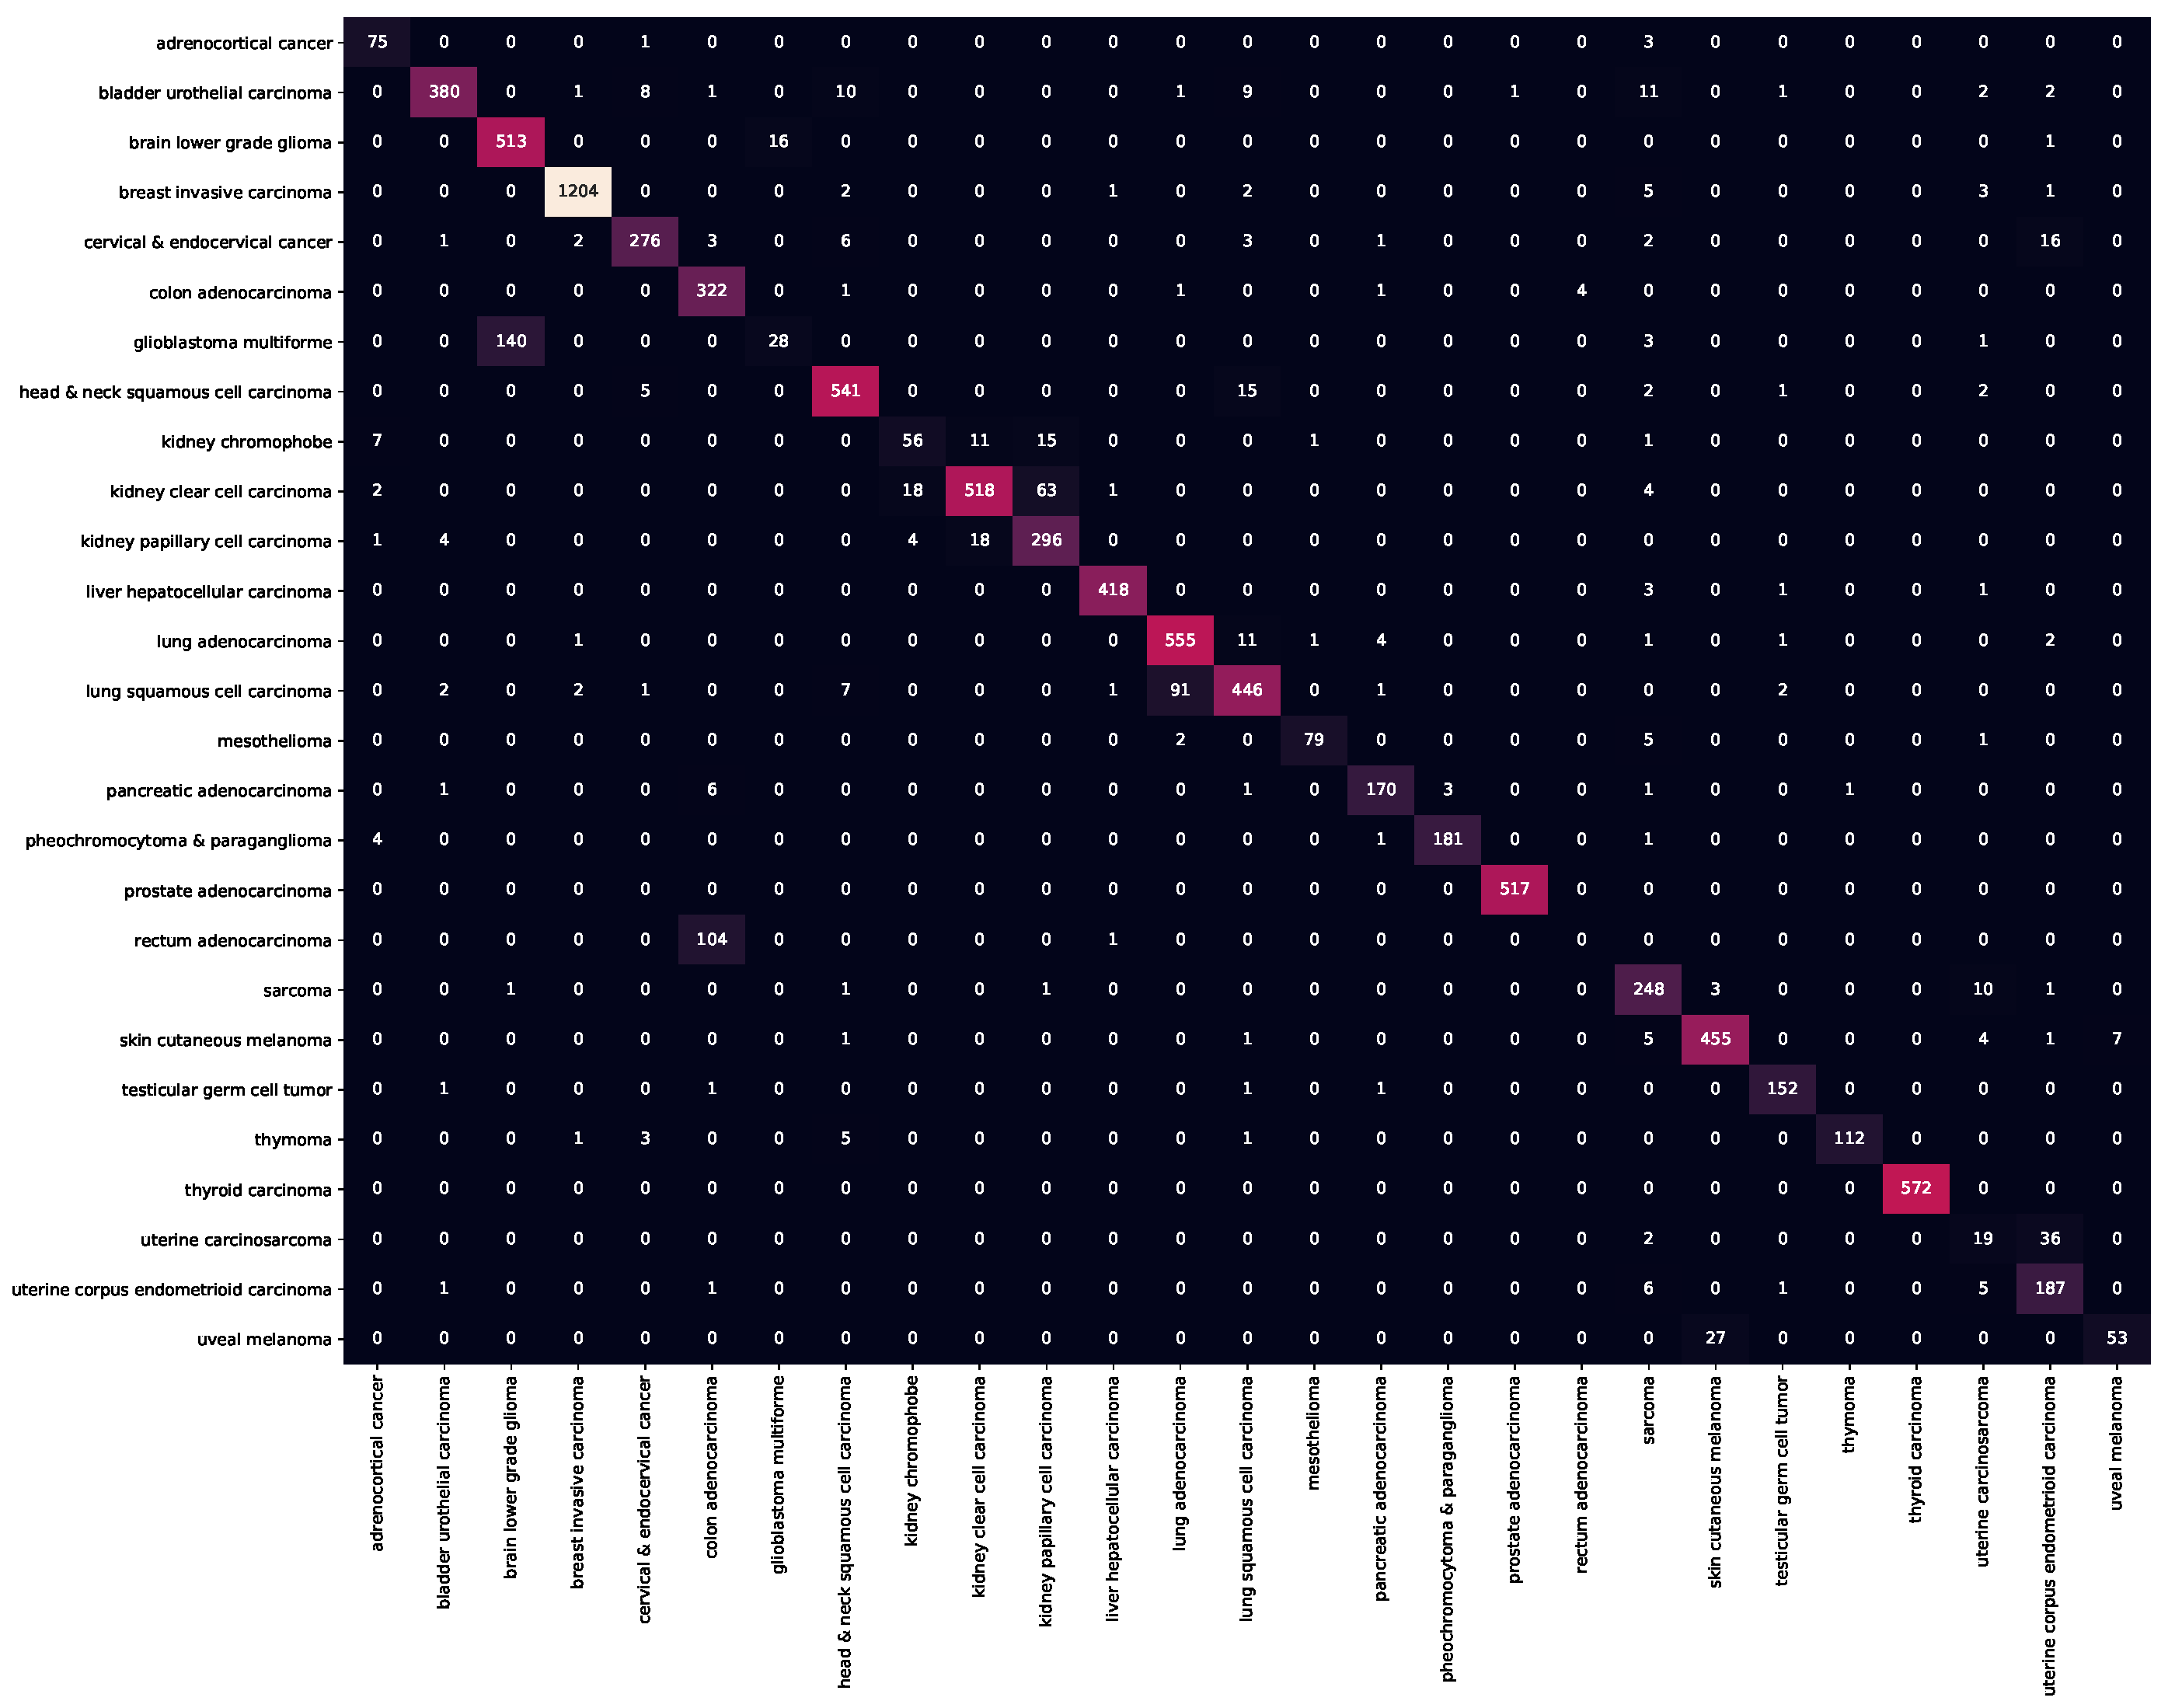
\includegraphics[scale=0.4, angle=90]{figs/m2_tcga_minmax_m2_100.pdf}
  \caption{Confusion matrix for M2 model with 100 labels}
\end{figure}

\begin{figure}[H]
  \centering
  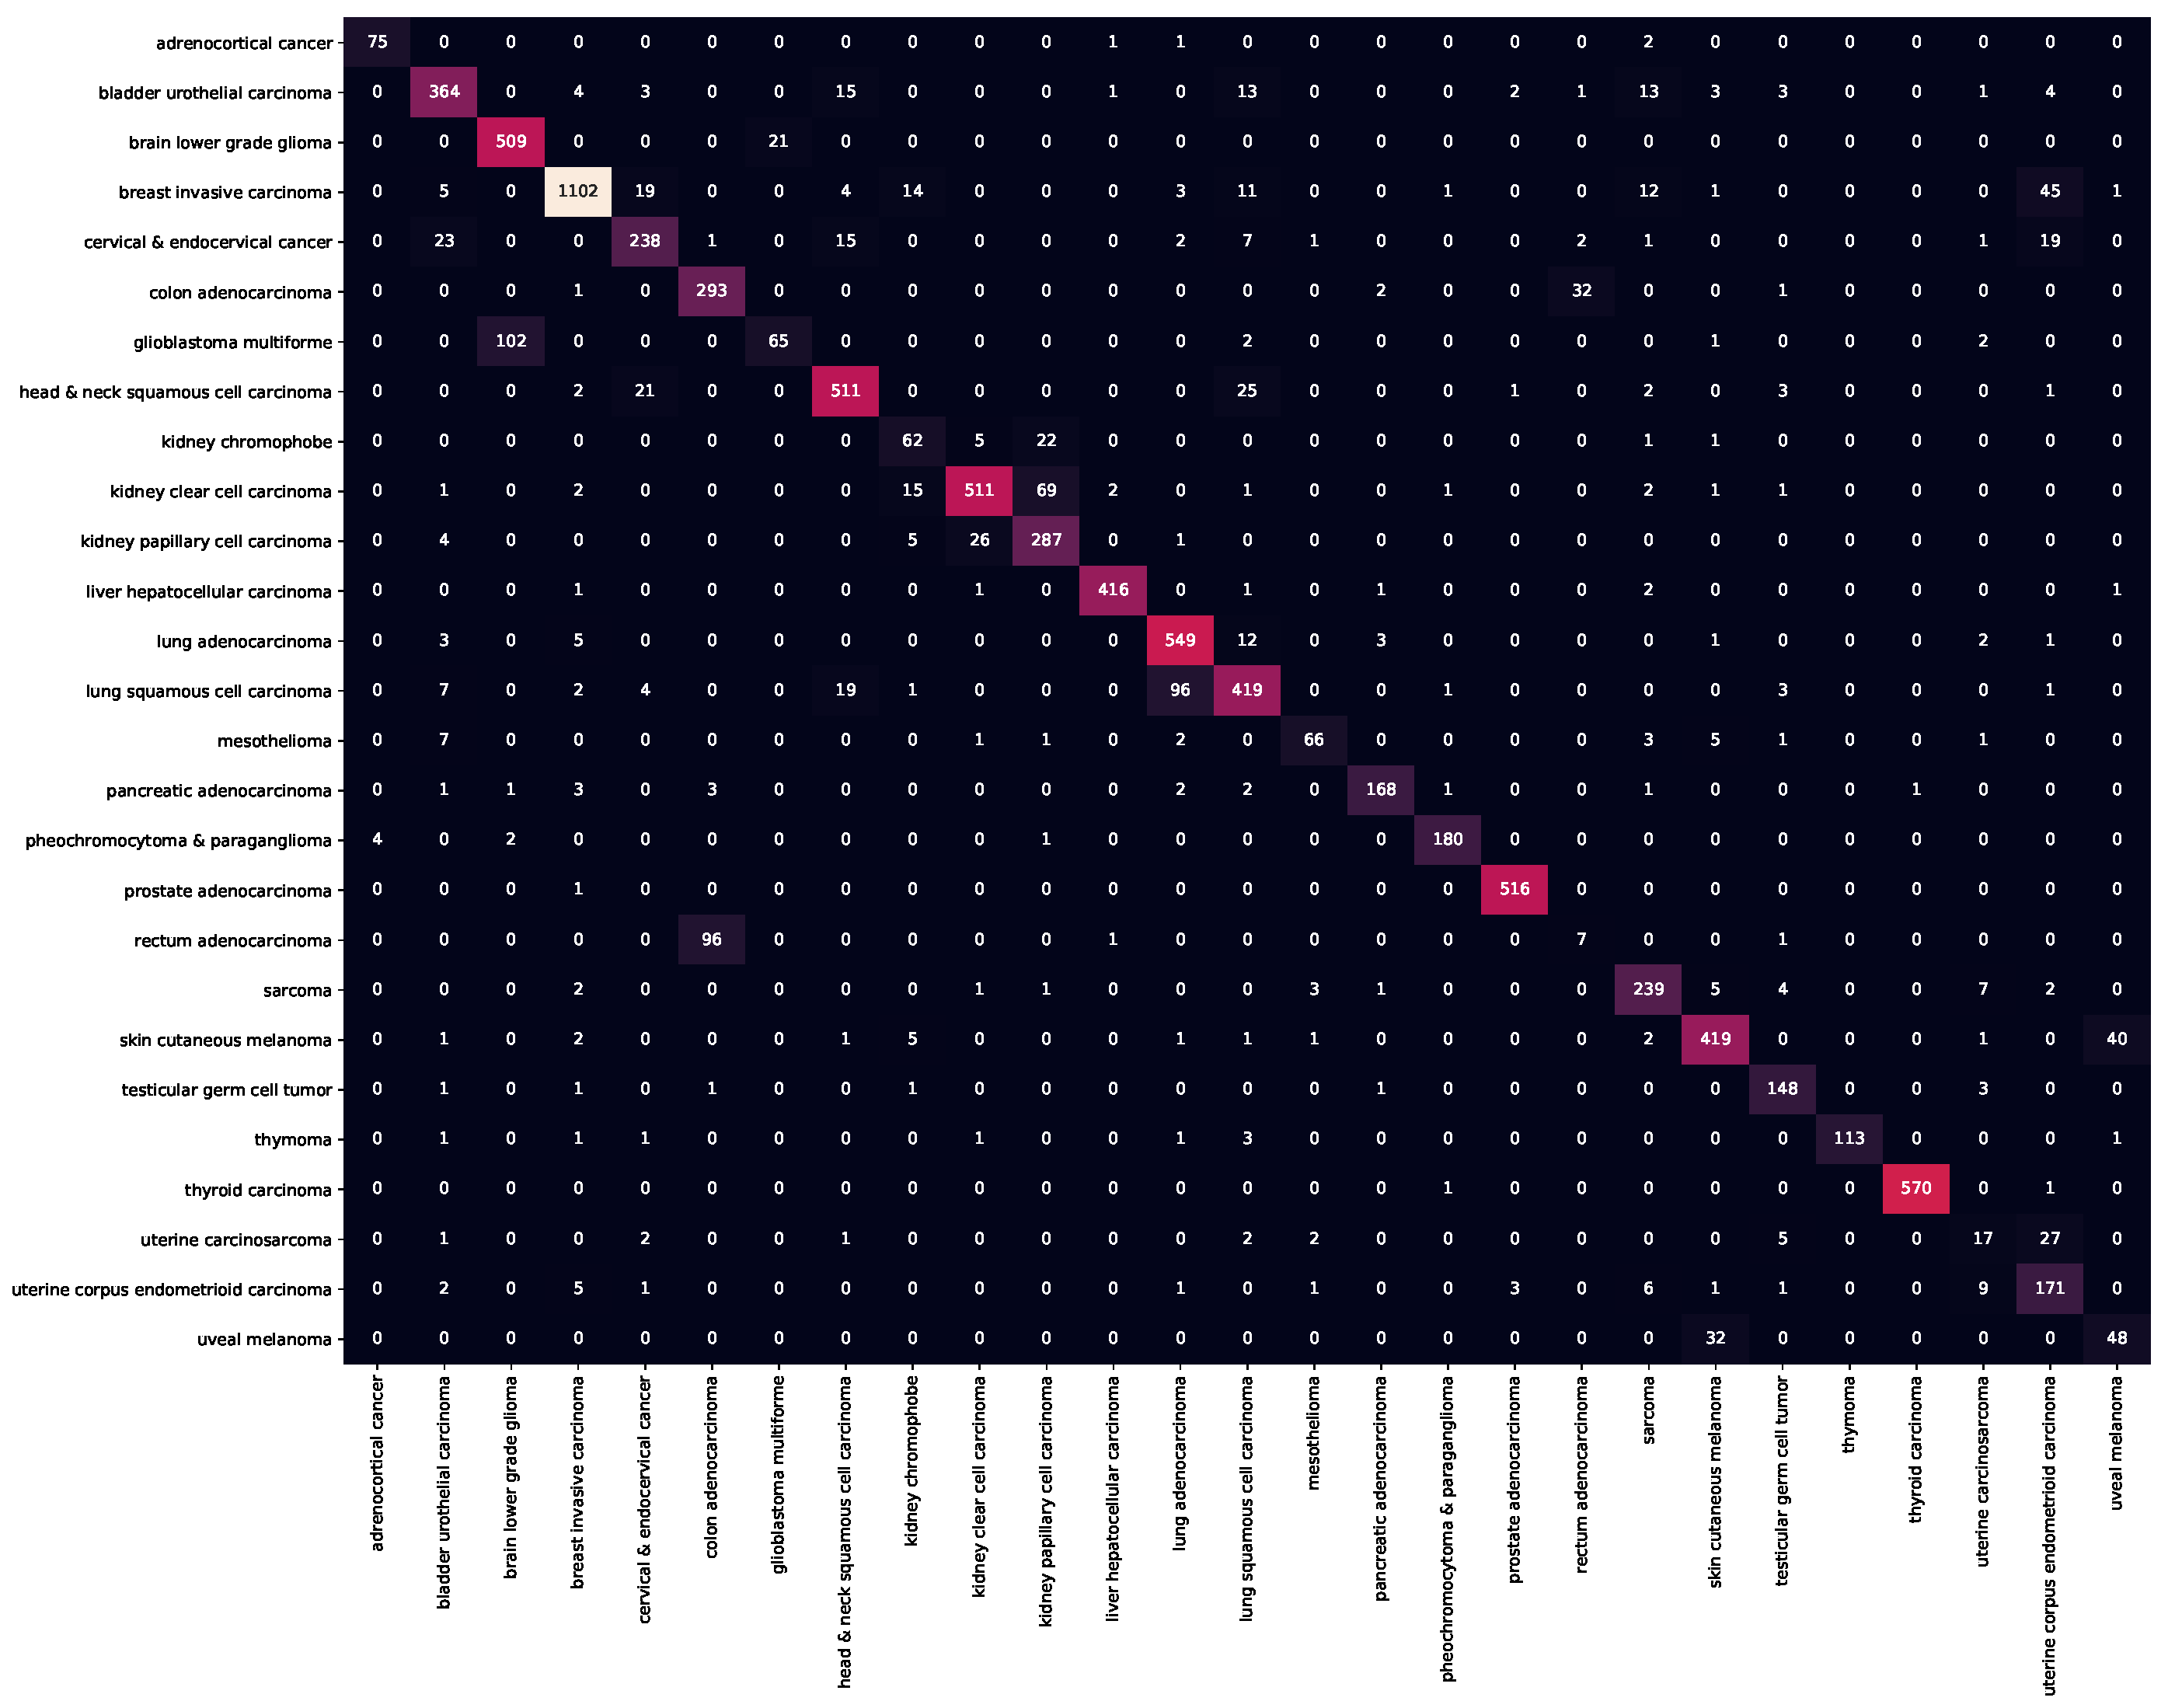
\includegraphics[scale=0.4, angle=90]{figs/ladder_tcga_standard_100.pdf}
  \caption{Confusion matrix for the ladder model with 100 labels}
\end{figure}

\chapter{Project Proposal} \label{proposal}
% Note: this file can be compiled on its own, but is also included by
% diss.tex (using the docmute.sty package to ignore the preamble)
\documentclass[12pt,a4paper,twoside,openany]{article}
\usepackage[pdfborder={0 0 0}]{hyperref}
\usepackage[margin=25mm]{geometry}
\usepackage{graphicx}
\usepackage{parskip}

\begin{document}

\begin{center}
\Large
Computer Science Tripos -- Part II -- Project Proposal\\[4mm]
\LARGE
A tool for phenotype prediction from cell genotype

\large
C.~London, Trinity College

Originator: Prof P.~Li\'o \& H.~Andres~Terre

19 October 2018
\end{center}

\vspace{5mm}

\textbf{Project Supervisor:} Prof P.~Li\'o \& H.~Andres~Terre

\textbf{Director of Studies:} Prof F.~Stajano

\textbf{Project Overseers:} Prof J.~Daugman  \& Dr A.~Madhavapeddy

% Main document

\section*{Introduction}

Phenotype prediction from cell genotype is an important problem in the field of bioinformatics, with usages in agriculture (for selecting crops with highest yield potential), medicine (for predicting likelihood of diseases/mutations), research, and many other fields. With the decreasing cost of genome sequencing this is becoming far more feasible for use in both research and the private sector.

Deep learning techniques provide an opportunity for generating high accuracy predictions of the phenotype from the genotype and as such much research in this area uses techniques such as autoencoders and neural networks to attempt to do this. However, much of the state of the art research is focused on generating predictions for only one type of cell, and so the network is structured specifically towards this cell. This is then not generalisable and not useful in other scenarios.

This project aims to build a tool that will provide these high accuracy predictions and is generalisable to data from different cells. By providing genotype data tagged with the observed phenotype for training, a user should then be able to use this tool to predict the required phenotype.

\section*{Starting point}

\subsection*{Prior Research}

This project is based on similar state of the art work done in papers on DeepGS\cite{DeepGS} (genomic selection) and DeepMetabolism\cite{DeepMetabolism}.

DeepGS was used to predict several phenotypes (grain length, grain hardness, plant height and more for wheat) when given genomic markers, and is now available as an R library. However the method  uses convolution and sampling to reduce data dimensionality, whereas the DeepMetabolism uses unsupervised pre-training in the form of an autoencoder to speed the supervised learning up. I believe that this is the better way to do it, and prescribes a less rigid structure on the model.

DeepMetabolism was used to predict three phenotypes of \textit{Escherichia Coli} and uses unsupervised pre-training with an autoencoder. However the autoencoder is used for denoising purposes, and the output, a cleaned version of the input data, is used for predictio instead of using the latent representation. The autoencoder is also structured specifically to correspond to the genome and proteins of \textit{E. Coli} and so the re-usability is limited.

\subsection*{Libraries and codebase}

The code for the learning will be written in Python, because Python has excellent support for advanced deep learning libraries. I have written machine learning code in Python before using Scikit-learn, but for this project I will use either Tensorflow or PyTorch as these libraries provide much better support for deep learning applications, as well as allowing for data parallelism and therefore large speed-ups when running on a GPU.

\section*{Resources required}

For this project I shall mainly use my own laptop, a 2014 Macbook Pro with a dual core Intel i5, 8GB of RAM and 128GB of flash storage. Source code for the project will be kept in a Git repository that will be synced with a repository on Github. The \LaTeX\\ source will be stored on my machine, and backed up to both overleaf.com and Google Drive. The entire content of my laptop will be frequently backed up to an external 500GB HDD.

The training of the model will be done using GPUs that can be provided by the Computer Lab, with confirmation from Professor Li\'o.

Data for training and testing the model will be both artificially generated as part of the project, and provided by the Plant Sciences department.

\section*{Work to be done}

\subsection*{Reading and further research}

\begin{itemize}
    \item Re-read papers on DeepGS and DeepMetabolism looking for particular insight into the exact models used to see ways they could be improved.
    
    \item Deep learning to model the hierarchical structure of the cell[3] - this is less relevant to the project as it involves a neural network that is pre-structured by hand, but still involves genotype-phenotype prediction and so may contain useful insights.
    
    \item Principles of gene manipulation and genomics\cite{Genomics} Chapters 16 to 20 - a book about genome analysis, involving genomic and transcriptomic data. This is necessary because I have never worked on a project with large scale genome analysis before.
    
    \item Reducing the dimensionality of data using neural networks\cite{Encoders} - information on reducing the dimensionality of data using autoencoders.
    
    \item Sparse autoencoders (lecture notes by Andrew Ng) - more information about using autoencoders to learn the most important features of data unsupervised.
    
    \item Meetings with Prof. Haseloff - Prof. Haseloff is a member of the plant sciences department here at the university and has experience working with the Computer Lab on other bioinformatics projects. He should be able to provide real data to use in training, as well as insight into what the synthetic data should look like.
    
\end{itemize}

\subsection*{The model}

The model for predicting the phenotype will be split into unsupervised and supervised portions.

The unsupervised portion is used to for dimesionality reduction of data, and is effectively a sort of pre-training for the model. Genomic data can be very large depending on the cell and so reducing the dimensionality to only the most important features should significantly speed the model up, and should hopefully provide greater prediction accuracy. This pre-training is likely to involve passing the genomic data into an autoencoder. An autoencoder is made up of two parts, an encoder and a decoder. The encoder includes the input layer and some hidden layers culminating in a final layer that has fewer nodes than the input layer. This layer is the latent representation of the input data. The decoder then attempts to reconstruct the input data from this representation, and backpropagation is performed to get the reconstruction as close as possible to the original. This latent representation should then be the features of the data that are most important for accurate reconstruction, and is therefore a reduced dimensionality representation of the data.

The supervised portion of the model will take the form of a neural network that takes in this latent representation as input and outputs the predicted phenotype. Backpropagation is performed to train the network to accurately predict the phenotype.

An important feature of the model should be the ability to work with different sized inputs and outputs. For the model to be generalisable to different cells, it will have to be able to take variable sized genome inputs, as the length of a genome sequence varies greatly between organisms. The output size will also not always be constant as the phenotype can take many forms - sometimes it might simply be a number e.g. if the studied phenotype is plant height, whereas other times it could be a class, or, as written in the extensions below, a photograph.

\paragraph{Testing.}

Testing the model will first be done with synthetic data, to ensure that it is working as it should i.e. recognising patterns and correctly identifying the most important features in the data, and the phenotype that should be associated with a given latent representation. The generation of this synthetic data will form an early part of this project, and will be done with input from Prof. Haseloff as he has significant experience with biological data.  

Once this is completed the model will then be trained and tested on real world data to verify its accuracy and usefulness as a real world prediction tool.

\subsection*{The tool}

This project should lead to a tool that can be used to predict phenotype without requiring users to know much about the underlying machine learning. To that end the tool should provide a basic front-end where users can add a file with training data, and, once training has completed, provide data that they want predictions for. The difficulty here is dealing with the different phenotypes a user might want, and having a model that can handle very different output requirements.

\section*{Success criteria}

Evaluation of the success of the project will be based upon the following criteria:

\begin{itemize}
    \item Better prediction accuracy than supervised training alone on a synthetic dataset (generated as part of the project) - compare the predicted phenotype with the synthetic phenotype generated for a particular pattern in the synthetic genotype data.
    \item Better prediction accuracy than supervised training alone on real world genotype and phenotype data.
    \item Producing a tool with a front-end that takes a file-path and trains the model based on the data within the file.
\end{itemize}

Prediction accuracy can be compared using a statistical significance test. The models will be trained on the same dataset and then tested on data that was not part of the training set. With synthetic data it is easy to generate data that was not part of the training set. With real world data if there is not enough for a separate training set and test set k-fold cross-validation can be performed.

\section*{Possible extensions}

If the main result is achieved and time is left some possible extensions are:

\begin{itemize}
    \item Use images of a cell/plant/etc. as the phenotype for training, and generate images as predictions. This would involve using other deep learning techniques to generate the images, likely generative adversarial networks.
    
    \item Measuring the importance of inputs to the output. Neural networks are often considered to be a sort of black box where input goes in and a result comes out. It is possible however to use some techniques to discover the importance of the input to the result. This can then be used to pinpoint which genes were most responsible for a certain phenotype. However, results can be misleading and the accuracy is not always good.
    
    \item Autoencoder structure based upon cell structure. Some well-studied organisms have extensive prior knowledge about gene interactions available in resources such as the Gene Ontology which would enabling structuring the autoencoder such that it partially mimics the cell. This should speed up training and could increase prediction accuracy. It would not be available for all cells, but if a user was using a well-studied cell the option to use a structured autoencoder would be useful.
\end{itemize}


\section*{Timetable}

Planned starting date is 20/10/2018.

\begin{enumerate}

\item \textbf{20/10/2018 -- 3/11/2018 } 

Perform the reading and research as stated in the "Work to be done" section. Install Tensorflow and PyTorch and decide which to use by doing small example learning tasks.

\item \textbf{4/11/2018 -- 18/11/2018} 

Write Python code to generate synthetic data for training. Begin building unsupervised model. Begin writing Introduction and Preparation chapters of dissertation.

\item \textbf{19/11/2018 -- 3/12/2018} 

Train and tune unsupervised model on synthetic data. Ensure that features expected to be important have large impact. Begin building supervised model. Begin writing Implementation chapter of dissertation.

\item \textbf{Michaelmas vacation} 

Do supervised training using output from the unsupervised model as input to the network. Make sure model is generalisable to different sized inputs and outputs corresponding to different cells and phenotypes.

\textbf{Milestones:}
\begin{itemize}
    \item Have a working prediction model trained on the synthetic data.
    \item Have finished writing dissertation Introduction and Preparation chapters.
\end{itemize}

\item \textbf{15/01/2019 -- 29/01/2019} 

Write progress report. Compare accuracy of model against a simple supervised model on artificial data to ensure model has better accuracy. Begin writing Evaluation chapter of dissertation.

\item \textbf{30/01/19 -- 13/02/19} 

Train model on real data and compare prediction accuracy with only supervised network.

\textbf{Milestones:}
\begin{itemize}
    \item Progress report submitted on 01/02/19.
\end{itemize}

\item \textbf{14/02/19 -- 28/02/19} 

Build a front-end that allows a user to pass a file of training data and create a model. Begin Extension 1: using images as phenotype.

\textbf{Milestones:}
\begin{itemize}
    \item Have a working tool allowing users to provide their own data for training.
    \item Have completed the Implementation chapter of the dissertation.
\end{itemize}

\item \textbf{01/03/19 -- 15/03/19} 

Extension 2: Pinpointing genes that have the greatest effect on phenotype.
Ensure full evaluation of all success criteria. Begin writing dissertation Evaluation chapter.

\item \textbf{Easter vacation}  

Writing dissertation and finishing any ongoing extensions. Extension 3 if time allows.

\item \textbf{23/04/19 -- 7/5/19} 

Proof reading, performing any final changes recommended by supervisor, preparing for submission in order to focus on exams.

\textbf{Milestone:} Have a completed and checked dissertation.

\end{enumerate}

\begin{thebibliography}{}
\bibitem{DeepGS} 
Ma W. \& Qiu Z. (2017) \textit{DeepGS: Predicting phenotypes from genotypes using Deep Learning}
\bibitem{DeepMetabolism}
Guo W., Xu Y. \& Feng X. (2017) \textit{DeepMetabolism: A Deep Learning System to Predict Phenotype from Genome Sequencing}
\bibitem{CellStructure}
Ma J., Yu M., Fong S., \& Ideker T. (2018) \textit{Using deep learning to model the hierarchical structure and function of a cell}
\bibitem{Genomics}
Primrose S. \& Twyman R. (2006) \textit{Principles of Gene Manipulation and Genomics}
\bibitem{Encoders}
Hinton G. \& Salakhutdinov R. (2006) \textit{Reducing the Dimensionality of Data with Neural Networks}

\end{thebibliography}

\end{document}